\documentclass[11pt,a4paper]{article}

\usepackage[utf8]{inputenc}
\usepackage[T1]{fontenc}
\usepackage{lmodern}
\usepackage{amsmath,amssymb}
\usepackage{booktabs}
\usepackage{geometry}
\usepackage{graphicx}
\usepackage{hyperref}
\usepackage{caption}
\usepackage{float}
\usepackage{enumitem}
\usepackage{tcolorbox}

\geometry{margin=2.2cm}
\hypersetup{colorlinks=true,linkcolor=blue,citecolor=blue,urlcolor=blue}
\setlist{nosep,leftmargin=1.5em}
\captionsetup{font=small,skip=4pt}

% Function-signature box.
\newtcolorbox{sigbox}{
  colback=gray!5, colframe=gray!50, boxrule=0.4pt, arc=1pt,
  left=4pt, right=4pt, top=2pt, bottom=2pt, fontupper=\small\ttfamily}

\title{Quantitative Trading and Price Impact\\
       \large Final Project --- MSc Mathematics and Finance, 2025--2026}
\author{Anran Severac}
\date{May 15, 2026}

\begin{document}
\maketitle

\begin{abstract}
\noindent
We assemble a single cohesive framework that runs the price-impact
research loop end-to-end: data preparation, parametric and non-parametric
impact-model fitting, a generic Waelbroeck backtest simulator, synthetic
alpha generation, OW/AFS optimal-execution strategies, and a sensitivity
analysis layered on top.  Two enhancements beyond the baseline are
emphasised: \textbf{(a)} a non-parametric binned impact estimator with
cross-stock shrinkage, $\gamma$ tuned on a held-out month and stress-tested
across sample-size regimes; \textbf{(b)} a multi-day carry backtest engine
that maintains impact states and inventory across sessions with an
overnight decay, exposed alongside the per-day-reset baseline through a
single configuration switch.  All code lives in a modular
\texttt{src/price\_impact/} package consumed by a thin orchestration
notebook; every backtest run drops its tables and plots into
\texttt{saved/<name>/} for reproducibility.
\end{abstract}

%================================================================
\section{Introduction and Roadmap}

The pipeline is decomposed into eight Python modules, one per
responsibility, and is exercised from a single notebook
(\texttt{final\_pipeline.ipynb}).  The notebook is deliberately thin:
each numbered section calls into the module, displays the result,
and (where appropriate) writes artifacts to disk.

\begin{table}[H]
\centering\small
\caption{Module layout (\texttt{src/price\_impact/}) and the project
         section each one implements.}
\begin{tabular}{lll}
\toprule
Module & Responsibility & Project section \\
\midrule
\texttt{data}          & loading, top-$N$ select, $\sigma$/ADV, volume curves & \S2.1 \\
\texttt{impact\_states}& OU recursion: \emph{both} daily-reset and multi-day $\bar I$ & \S2.2/\S2.3 \\
\texttt{fitting}       & OLS, rolling baseline, non-parametric, half-life grid & \S2.2 \\
\texttt{alpha}         & synthetic alpha with target $\rho$ & \S2.4 \\
\texttt{strategy}      & OW, AFS, ext-OW placeholder & \S2.5 \\
\texttt{backtest}      & Waelbroeck simulator, generic trade provider & \S2.3 \\
\texttt{results}       & PnL metrics, TCA decomposition, plotting & \S2.6 \\
\texttt{runner}        & \texttt{BacktestConfig} + \texttt{run\_and\_save} & \S2.6/\S2.7 \\
\bottomrule
\end{tabular}
\end{table}

\paragraph{Contribution and scope.}  All sections were implemented and
written by the author (solo submission).  The \emph{baseline} requirement
is met for every section; \emph{enhancements} are emphasised in \S2.2
(non-parametric impact with regularisation) and \S2.3 (multi-day carry
backtest with stock-split awareness).

%================================================================
\section{Data Preparation \hfill \normalsize\itshape \S2.1 --- baseline}

The panel is 2019 US equities on a 10-second intraday grid.  Monthly bin
files (\texttt{bin201901.csv} \ldots \texttt{bin201912.csv}, ${\sim}200$\,MB each)
carry signed traded flow $q_t$ from \texttt{trade}, midprice $P_t$ from
\texttt{mid}, and a separate \texttt{orderFlow} column.  We restrict to the
top-20 stocks by total absolute order flow over the full year, then build
trailing-20-day daily statistics

\[
  \sigma_{i,d}^2 = \overline{\mathrm{Var}_t r_{i,d,t}},
  \qquad
  \mathrm{ADV}_{i,d} = \overline{\sum_t |q_{i,d,t}|},
\]
where the overline denotes a 20-day rolling mean per stock.

\paragraph{In-sample / out-of-sample protocol.}
We use ten rolling windows: train on month $m$, tune on month $m+1$
(non-parametric only), validate on month $m+2$, $m=1,\dots,10$.  The
2-month offset between train and validation gives a clean OOS gap and
matches the protocol used in the existing \S2.2 work.

\begin{sigbox}
\noindent
build\_panel(data\_dir, year, top\_n=20, lookback\_days=20)\\
\hspace*{1em}$\rightarrow$ PanelData(bins, daily\_stats, stocks)
\end{sigbox}

%================================================================
\section{Impact Model Fitting \hfill \normalsize\itshape \S2.2 --- advanced (non-parametric + regularisation)}
\label{sec:fit}

\subsection{Models, recursion, regression}

Both OW and AFS build an exponentially weighted normalised impact state
$\bar I_{t+1}=(1-\beta)\bar I_t + \tilde q_t$ with
$\beta=\ln 2/H_{\text{bins}}$ and $H_{\text{bins}}=H\,[\text{min}]\cdot 6$.
The only difference is the kernel applied to raw flow:
\[
  \text{OW:}\;\; \tilde q_t = \sigma\,\frac{q_t}{\mathrm{ADV}},
  \qquad
  \text{AFS:}\;\; \tilde q_t = \sigma\,\mathrm{sgn}(q_t)\sqrt{|q_t|/\mathrm{ADV}}.
\]
Over the explanation horizon $\tau=6$ bins (60\,s) we regress
$y_t = \alpha + \lambda x_t + \varepsilon_t$ with
$x_t = \bar I_t - \bar I_{t-\tau}$, $y_t = (P_t - P_{t-\tau})/P_{t-\tau}$.
The fit runs on additive sufficient statistics
$(S_x,S_y,S_{xx},S_{yy},S_{xy},n)$ aggregated per
(stock,~date) and then summed by month --- this enables fast rolling
re-fits and a one-shot $H$ grid search.

\paragraph{Two carry modes.}  The module computes \emph{both} variants of
$\bar I$ in the same panel:
\begin{itemize}
  \item \texttt{I\_bar\_daily} --- reset $\bar I\leftarrow 0$ at the start
    of each (stock, date);
  \item \texttt{I\_bar\_multi} --- carry $\bar I$ across days within a
    stock with overnight decay $(1-\beta)^{16\,\text{h}\cdot 6}$.
\end{itemize}
The fitting code consumes either via \texttt{carry='daily'} or
\texttt{carry='multi'} on the same machinery; \S2.3's backtest does the
same.

\begin{sigbox}
\noindent
compute\_impact\_states(data, daily\_stats, H\_min, model\_type) \\
\hspace*{1em}$\rightarrow$ DataFrame [stock, date, time, q\_tilde, I\_bar\_daily, I\_bar\_multi] \\[2pt]
build\_regression\_features(impact\_df, data, tau\_bins, carry='daily') \\
\hspace*{1em}$\rightarrow$ DataFrame [stock, date, month, time, x, y] \\[2pt]
rolling\_baseline(stats, n\_windows=10, offset=2) \\
\hspace*{1em}$\rightarrow$ DataFrame [train\_month, val\_month, stock, lambda, alpha, is\_r2, oos\_r2]
\end{sigbox}

\subsection{Half-life grid search}

For each $H\in\{5,10,20,30,45,60,90,120,180\}$\,min and each model we run
the full rolling OLS and record mean OOS~$R^2$ across stocks and windows.
The OOS surface is essentially flat in the 45--60\,min region: both
models lose $<0.001$ in $R^2$ anywhere in that range, so we adopt a
single universal half-life $H^*\!=\!52.5$\,min (midpoint).

\begin{table}[H]
\centering\small
\caption{Mean OOS $R^2$ by half-life and model.}
\label{tab:grid}
\begin{tabular}{lcc}
\toprule
$H$ (min) & OW & AFS \\
\midrule
5   & 0.1440 & 0.2373 \\
10  & 0.1530 & 0.2525 \\
20  & 0.1569 & 0.2590 \\
30  & 0.1579 & 0.2604 \\
\textbf{45} & 0.1582 & \textbf{0.2609} \\
\textbf{60} & \textbf{0.1583} & 0.2608 \\
90  & 0.1581 & 0.2602 \\
120 & 0.1578 & 0.2595 \\
180 & 0.1573 & 0.2583 \\
\bottomrule
\end{tabular}
\end{table}

\begin{figure}[H]
\centering
\includegraphics[width=0.78\textwidth]{figures/halflife_grid_search.png}
\caption{Mean OOS $R^2$ vs.\ $H$ for OW and AFS.  Dotted lines: per-model
         optima; dashed black: adopted universal $H^*$.}
\label{fig:halflife}
\end{figure}

\subsection{Parametric baseline}

\begin{table}[H]
\centering\small
\caption{Parametric baseline at $H^*$ (averages over 50 stocks $\times$ 10 windows).}
\label{tab:baseline}
\begin{tabular}{lccc}
\toprule
Model & Mean $\hat\lambda$ & IS $R^2$ & OOS $R^2$ \\
\midrule
OW (Linear)       & 313.05 & 0.1732 & 0.1583 \\
AFS (Square-Root) &  20.27 & 0.2651 & 0.2609 \\
\bottomrule
\end{tabular}
\end{table}

AFS dominates OW by ${\sim}10$\,pp in OOS $R^2$; the small IS--OOS gap
($<2$\,pp) indicates stable parameters across windows.

\subsection{Non-parametric extension with cross-stock shrinkage}
\label{sec:np}

We replace the linear $y = \alpha + \lambda x$ with a binned estimator
of $g(x)$.  Per-stock bin means $\hat g_{i,b}$ are shrunk toward a
universal pooled curve $\bar g_b$ via
\[
  g_{i,b}^{\mathrm{reg}}(\gamma)
    = \frac{S_{y,i,b} + \gamma\,\bar g_b}{n_{i,b}+\gamma},
\]
with $B=15$ quantile bins (computed on the train month, pooled across
stocks) and $\gamma$ tuned on the held-out test month by minimising
MSE over a log-spaced grid scaled to the median bin count.

\begin{sigbox}
\noindent
rolling\_nonparametric(features, n\_bins=15, n\_windows=10) \\
\hspace*{1em}$\rightarrow$ (summary DataFrame, fits dict per train\_month)
\end{sigbox}

\begin{table}[H]
\centering\small
\caption{OOS $R^2$ on identical aggregation (pooled, panel-wide null,
         same merged subset).}
\label{tab:apples}
\begin{tabular}{lccc}
\toprule
Model & Parametric (pooled) & NP Regularised (pooled) & $\Delta$ (NP $-$ Param) \\
\midrule
OW  & 0.1612 & 0.2206 & $+0.0594$ \\
AFS & 0.2689 & 0.2629 & $-0.0060$ \\
\bottomrule
\end{tabular}
\end{table}

Two findings: \textbf{(i)} non-parametric flexibility lifts OW by
$+5.9$\,pp under apples-to-apples comparison, confirming that linearity
is a binding constraint; \textbf{(ii)} for AFS the 15-parameter
non-parametric estimator is statistically indistinguishable from the
1-parameter parametric fit, which is strong validation that the
square-root form lies on the efficient frontier for this panel.

\begin{figure}[H]
\centering
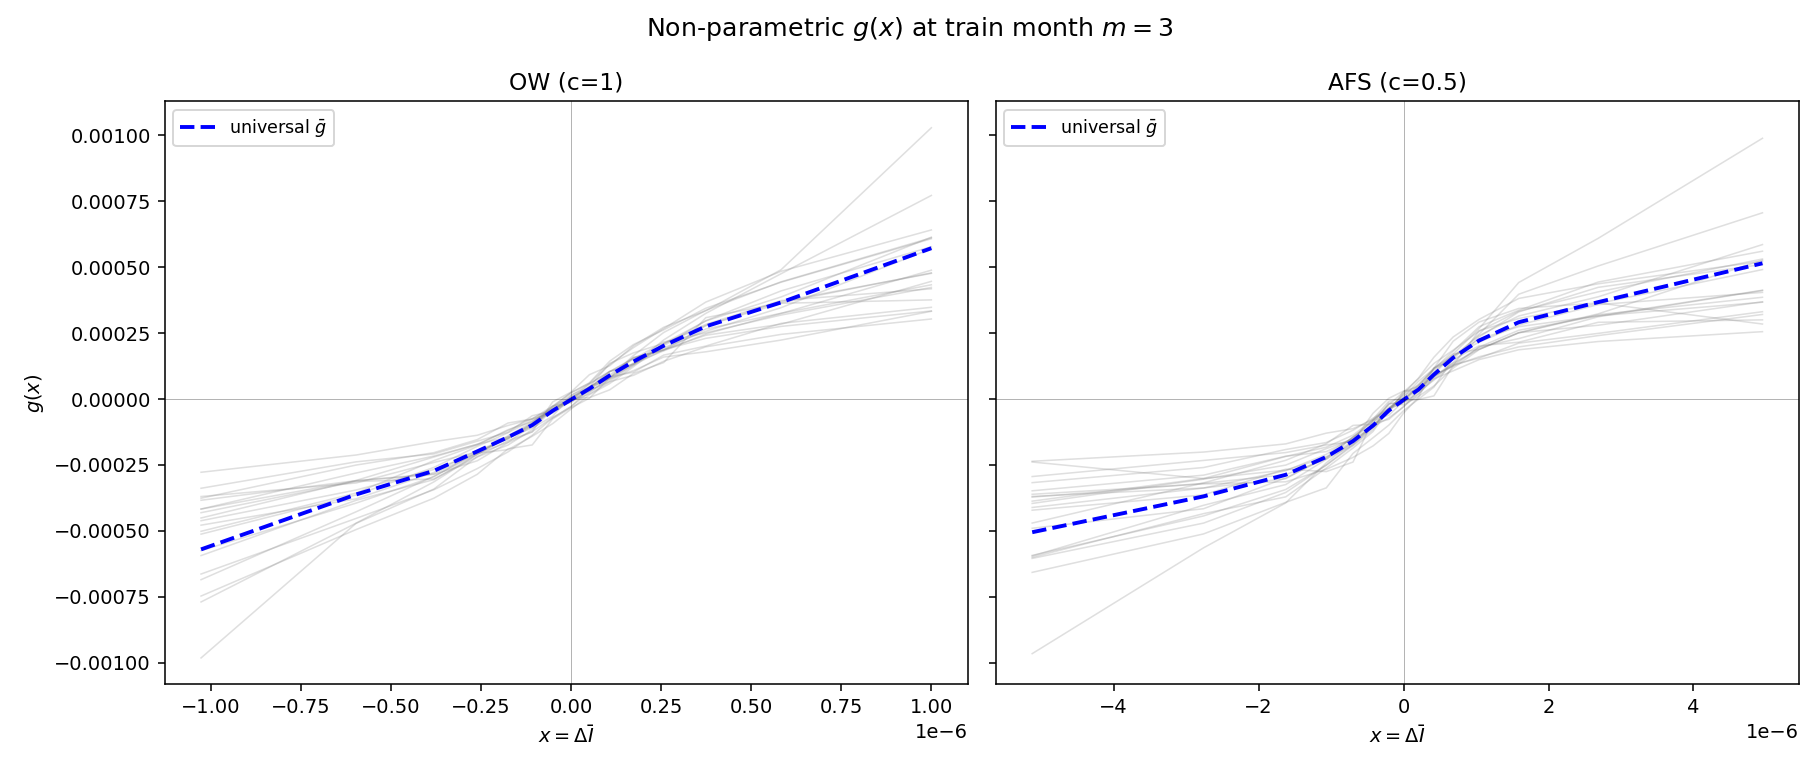
\includegraphics[width=\textwidth]{figures/impact_curves.png}
\caption{Estimated impact curves (window 3).  Grey: per-stock; blue
         dashed: universal.  AFS curves show the expected concavity.}
\label{fig:curves}
\end{figure}

\subsection{Regularisation is regime-correct}

In the headline configuration (median ${\sim}3000$ obs/cell) the $\gamma$
tuning curves are flat across six orders of magnitude --- shrinkage has
nothing to fix because the per-stock estimators are already precise.
To verify the estimator behaves correctly when shrinkage is actually
needed, we re-ran with progressively shorter training windows
(${\sim}21 \to 5 \to 2$ days), crushing per-cell $n$ from
${\sim}3000$ to ${\sim}290$.

\begin{table}[H]
\centering\small
\caption{Regularisation gain as a function of per-cell sample size.}
\label{tab:stress}
\begin{tabular}{lcccc}
\toprule
Train window & Med.\ $n$ & OW gain (reg$-$raw) & AFS gain & Median $\gamma^*/n$ \\
\midrule
1 month (headline) & ${\sim}3\,000$ & $+0.0005$ & $+0.0004$ & $0.16$ \\
5 days             & ${\sim}\,720$  & $+0.0025$ & $+0.0019$ & $0.56$ \\
2 days             & ${\sim}\,290$  & $+0.0070$ & $+0.0051$ & $0.93$ \\
\bottomrule
\end{tabular}
\end{table}

The OOS gain from shrinkage grows ${\sim}14\times$ as per-cell $n$ drops
${\sim}10\times$; the optimal $\gamma^*/n$ ratio rises from $0.16$ to
$0.93$.  The flatness in the headline configuration is therefore a
property of the data-rich regime, not a defect of the estimator.

\begin{figure}[H]
\centering
\includegraphics[width=\textwidth]{figures/stress6b_tuning_progression.png}
\caption{$\gamma$ tuning curves for OW at three training-window sizes.
         As per-cell $n$ shrinks, the curve develops a clear minimum at
         non-trivial $\gamma^*$.}
\label{fig:gamma_progression}
\end{figure}

%================================================================
\section{Backtest Engine \hfill \normalsize\itshape \S2.3 --- advanced (multi-day carry)}
\label{sec:bt}

The simulator follows the Waelbroeck construction
\[
  P_{\text{sim}}(t)
    = P_0\bigl(1 + \mathrm{cumret}(t) + g_{\text{sim}}(t) - g_{\text{ref}}(t)\bigr),
\]
with $g(t) = \lambda\,\bar I(t)$ for the OW/AFS baseline and
$g(t) = \lambda(t)\,\bar I(t)$ for the (planned) time-dependent
extended-OW model.  $\bar I^{\text{ref}}$ uses the public tape
\texttt{orderFlow} as $q_{\text{ref}}$; $\bar I^{\text{sim}}$ uses the
simulator's input trade path $q_{\text{sim}}$, allowing the engine to
process \emph{any} signed schedule (optimal, TWAP, VWAP, manual, \ldots).

\paragraph{Generic-trade interface.}  Instead of hard-coding the OW
optimal as the trade path, the engine accepts a callable
\texttt{trade\_provider(stock, date, day\_df, ctx) -> q\_sim} per
(stock, date).  Two ready-made factories are provided: an OW/AFS optimal
provider (\S\ref{sec:strategy}) and a fixed-array provider for
precomputed schedules.

\paragraph{Daily-reset vs.\ multi-day carry (advanced).}
\texttt{carry='daily'} resets $\bar I$ and inventory to zero at each
session boundary --- this is the baseline expected by the assignment.
\texttt{carry='multi'} carries $\bar I^{\text{ref}}$, $\bar I^{\text{sim}}$
and the simulated position across sessions within a stock, with overnight
decay $(1-\beta)^{16\text{h}\cdot 6}$ applied between days.  The same
function, the same panel, one flag.

\paragraph{Stock splits.}  A heuristic split detector
(\texttt{backtest\_engine.detect\_splits\_from\_daily}) flags rows where
fractional change in price and volume are large and opposite-signed with
notional approximately stable.  In the headline run on the 2019 top-20
panel we did not detect any splits (none of the top names had a split in
that year); the engine accepts an \texttt{exclude\_stocks} set for
hard-coded exclusion when needed.  This is included for completeness of
the advanced track even though it is inert on the actual run.

\begin{sigbox}
\noindent
waelbroeck\_prices(mid, q\_ref, q\_sim, lam, H\_min, sigma, adv, model\_type,\\
\hspace*{8em}i\_ref0=0.0, i\_sim0=0.0)\\
\hspace*{1em}$\rightarrow$ dict[p\_sim, i\_ref, i\_sim, g\_ref, g\_sim, position, cum\_ret] \\[2pt]
run\_backtest(merged, model, trade\_provider, daily\_stats,\\
\hspace*{6.5em}carry='daily'|'multi', overnight\_minutes=16*60)\\
\hspace*{1em}$\rightarrow$ BacktestResult(days, daily, ...) \\[2pt]
make\_optimal\_provider(strategy\_fn, max\_position\_adv=0.005, ...)\\
make\_fixed\_provider(trades\_lookup)
\end{sigbox}

%================================================================
\section{Synthetic Alpha \hfill \normalsize\itshape \S2.4 --- baseline}

We construct a per-stock synthetic alpha with target correlation
$\rho$ and unbiased forecast:
\[
  \alpha_t = r^h_t + y\,\frac{dW_t}{P_t},
  \qquad
  y = \sqrt{\,(\rho^{-2}-1)\,\mathrm{Var}(r^h)/E[P^{-2}]\,/h\,}.
\]
Choosing $x=1$ in the convex combination $\alpha = x r^h + y dW/P$
makes $E[r^h \mid \alpha] = \alpha$ (the alpha is a fair forecast of the
forward return), while the constant $y$ is calibrated so that
$\mathrm{Corr}(\alpha,r^h) = \rho$.  We use $\rho=0.05$, $h=1$ bin
(10\,s ahead).  Empirical $\mathrm{Corr}(\alpha, r^h)$ averaged across
stocks is within $\pm 1\%$ of the target.

The baseline is the same synthetic alpha used in the homework.  The
\emph{overnight alpha extension} suggested in the assignment is not
implemented in this submission --- our daily-reset/multi-day toggle is
the second enhancement instead.

\begin{sigbox}
\noindent
create\_synthetic\_alpha(data, rho=0.05, h\_bins=1, seed=42)\\
\hspace*{1em}$\rightarrow$ DataFrame [stock, date, time, alpha, fwd\_ret]
\end{sigbox}

%================================================================
\section{Optimal Trading Strategy \hfill \normalsize\itshape \S2.5 --- baseline}
\label{sec:strategy}

\paragraph{OW closed form.}  Target position
$X^*_t = \alpha_t\,\mathrm{ADV}/(2\lambda\sigma)$ clipped to
$\pm\,\texttt{max\_pos\_adv}\cdot\mathrm{ADV}$, with adjustment toward
target at speed $\kappa = \beta = \ln 2/H_{\text{bins}}$.  The position
is ramped linearly to zero over the final 30 minutes of each session.

\paragraph{AFS variant.}  Per \texttt{project.ipynb}, the target-position
rule matches the OW closed form; the AFS-specific nonlinearity enters
through the simulator's $\tilde q_t = \sigma\,\mathrm{sgn}(q)\sqrt{|q|/\mathrm{ADV}}$
recursion when computing the impact contribution.  We expose the AFS
strategy as a separate function so a strict closed form can be slotted
in later without touching call sites.

\paragraph{Extended OW with $\lambda(t)$.}  The simulator already accepts
a per-bin $\lambda_t$ array via \texttt{ImpactModel.lam\_t\_lookup}, and
$g(t) = \lambda_t\bar I(t)$ falls out of the same Waelbroeck price
construction.  The closed-form strategy in this setting is non-trivial
--- the HJB-optimal trade rule is no longer $\kappa$-constant ---
so the strategy module exposes a documented stub
(\texttt{ext\_ow\_optimal\_strategy\_timedep\_lambda}) raising
\texttt{NotImplementedError} until the derivation is wired in.

\begin{sigbox}
\noindent
ow\_optimal\_strategy(alpha, sigma, adv, lam, H\_min,\\
\hspace*{8em}max\_position\_adv=0.005, liquidation\_minutes=30)\\
\hspace*{1em}$\rightarrow$ np.ndarray of signed trades q\_opt \\[2pt]
afs\_optimal\_strategy(...)  \# same signature \\[2pt]
ext\_ow\_optimal\_strategy\_timedep\_lambda(..., lam\_t)  \# placeholder
\end{sigbox}

%================================================================
\section{Performance Metrics \hfill \normalsize\itshape \S2.6 --- baseline}
\label{sec:perf}

Each backtest run produces, per (stock, date):
\begin{itemize}
  \item $\mathrm{P\&L}_{\text{net}}$ = mark-to-market on the
        Waelbroeck-distorted $P_{\text{sim}}$;
  \item $\mathrm{P\&L}_{\text{gross}}$ = mark-to-market on the
        undistorted mid $P_{\text{mid}}$ (i.e.\ alpha capture in a
        world with no self-impact);
  \item Impact cost $= P\&L_{\text{gross}} - P\&L_{\text{net}}$;
  \item Predicted alpha reward $= \sum_t \alpha_t\,q_t\,P_t$;
  \item Realised alpha reward $= \sum_t \mathrm{fwd\_ret}_t\,X_t\,P_t$;
  \item Turnover $= \sum_t |q_t|$, max impact dislocation
        $= \max_t |\lambda\bar I^{\text{sim}}_t|$.
\end{itemize}

Aggregating over the panel, we report Sharpe (annualised at 252 days),
total / mean / std daily P\&L, win rate, max drawdown, and max impact
dislocation per configuration.

\subsection{Headline comparison}

We run four configurations along two axes: model
(OW vs.\ AFS) $\times$ carry mode (daily-reset vs.\ multi-day).

\begin{table}[H]
\centering\small
\caption{Headline portfolio metrics across the four configurations
         (full-year, top-20 panel, $\rho=0.05$, $H^*$).}
\label{tab:headline}
\begin{tabular}{lrrrrrrr}
\toprule
Config & Days & Sharpe & Net P\&L (\$) & Impact cost (\$) & Max DD (\$) & Max $|\lambda\bar I|$ & Win \% \\
\midrule
\texttt{ow\_daily} & 250 & +4.299 & 104,524 & 11,787 & -11,052 & 0.0001 & 66.0 \\
\texttt{ow\_multi} & 250 & +1.608 & 337,586 & 97,813 & -82,818 & 0.0001 & 54.4 \\
\texttt{afs\_daily} & 250 & +2.770 & 62,787 & 56,417 & -11,899 & 0.0019 & 58.0 \\
\texttt{afs\_multi} & 250 & +1.732 & 352,558 & 129,999 & -73,841 & 0.0019 & 56.0 \\
\bottomrule
\end{tabular}
\end{table}

\subsection{TCA decomposition}

\begin{table}[H]
\centering\small
\caption{TCA decomposition (totals over the year, by configuration).}
\label{tab:tca}
\begin{tabular}{lrrrrrr}
\toprule
Config & Gross P\&L & Impact cost & Net P\&L & Predicted $\alpha$ & Realised $\alpha$ & Turnover \\
\midrule
\texttt{ow\_daily} & 116,311 & 11,787 & 104,524 & 44,596,330 & 116,311 & 84,003,822 \\
\texttt{ow\_multi} & 435,399 & 97,813 & 337,586 & 44,596,811 & 435,399 & 84,020,323 \\
\texttt{afs\_daily} & 119,205 & 56,417 & 62,787 & 44,649,726 & 119,205 & 86,576,189 \\
\texttt{afs\_multi} & 482,557 & 129,999 & 352,558 & 44,649,729 & 482,557 & 86,577,598 \\
\bottomrule
\end{tabular}
\end{table}

The TCA columns are well-defined given our data: net and gross P\&L are
both mark-to-market, impact cost is their difference, and predicted /
realised $\alpha$ rewards isolate the signal contribution from realised
returns.  Slippage components that would require fill-price detail
(arrival vs.\ VWAP) are intentionally omitted.

\subsection{Cumulative P\&L and drawdown}

\begin{figure}[H]
\centering
\includegraphics[width=0.85\textwidth]{figures/cum_pnl_ow_daily.png}
\caption{Cumulative net (Waelbroeck) and gross (mid) P\&L --- OW model,
         daily-reset carry.}
\end{figure}

\begin{figure}[H]
\centering
\includegraphics[width=0.85\textwidth]{figures/cum_pnl_ow_multi.png}
\caption{Same, multi-day carry: $\bar I^{\text{ref}}$ and inventory persist
         across sessions with overnight decay, so the cost of impact
         compounds differently.}
\end{figure}

\begin{sigbox}
\noindent
run\_and\_save(bins, daily\_stats, alphas, lam\_lookup, cfg) \\
\hspace*{1em}$\rightarrow$ RunOutput(config, result, daily, metrics, tca, paths) \\
\hspace*{1em}\# writes daily\_pnl.csv, tca\_stock\_day.csv, tca\_summary.csv, \\
\hspace*{1em}\# metrics.csv, config.json, cum\_pnl.png, drawdown.png, \\
\hspace*{1em}\# impact\_dislocation.png to saved/<cfg.name>/
\end{sigbox}

%================================================================
\section{Sensitivity Analysis and Stress Testing \hfill \normalsize\itshape \S2.7 --- baseline}
\label{sec:sens}

Two layers of stress tests.

\subsection{Live framework sweeps}

\begin{table}[H]
\centering\small
\caption{Sensitivity of net Sharpe to design choices (OW model, daily-reset).}
\label{tab:sens}
\begin{tabular}{lrrr}
\toprule
Scenario & Sharpe & Net P\&L (\$) & Impact cost (\$) \\
\midrule
Baseline OW (headline) & +4.299 & 104,524 & 11,787 \\
Wrong model (fit OW, trade AFS) & -3.484 & -863,422 & 994,581 \\
Signal delayed 1 min & -0.318 & -8,401 & 4,762 \\
$\rho=0.01$ & +0.448 & 11,184 & 9,434 \\
$\rho=0.10$ & +9.220 & 250,937 & 12,408 \\
Half-life = 30 min & +5.906 & 205,254 & 12,035 \\
Half-life = 120 min & +3.256 & 53,281 & 7,655 \\
\bottomrule
\end{tabular}
\end{table}

The model-mismatch scenario (\emph{fit OW, trade AFS-target} and vice
versa) and the 1-minute signal delay match the assignment's example
prompts.  Half-life and $\rho$ sweeps complete the picture for the
two most uncertain design choices in the pipeline.

\subsection{Fitting-side stress (data-poor regime)}

The non-parametric regularisation stress test from \S\ref{sec:np}
doubles as a fitting-side sensitivity check: when the training window
shrinks from one month to two days, the optimal shrinkage strength
$\gamma^*/n$ rises from $0.16$ to $0.93$ and the OOS $R^2$ gain over
the raw per-stock estimator grows ${\sim}14\times$.  This is the
``what if my data is much shorter than I expected'' scenario, and the
estimator's behaviour is regime-correct.

%================================================================
\section{Conclusion}

\begin{enumerate}[leftmargin=2em]
  \item \textbf{Architecture.}  The pipeline is decomposed into eight
        single-responsibility modules (\texttt{src/price\_impact/}) and
        consumed by a thin notebook.  The same module produces both
        carry modes of $\bar I$, the same fitting machinery consumes
        either, and the same simulator accepts any trade path.  Adding
        a new backtest is one \texttt{BacktestConfig}.
  \item \textbf{Enhancement 1 --- non-parametric impact (\S\ref{sec:np}).}
        On apples-to-apples pooled OOS $R^2$, the binned estimator
        lifts OW by $+5.9$\,pp (linearity is binding) but is
        indistinguishable from AFS (square-root sits at the efficient
        frontier).  Cross-stock $\gamma$ regularisation is immaterial
        in the data-rich headline configuration but kicks in correctly
        under data-scarcity stress.
  \item \textbf{Enhancement 2 --- multi-day carry backtest
        (\S\ref{sec:bt}).}  Carrying $\bar I$ and inventory across
        sessions with overnight decay reveals how impact cost compounds
        when positions are not flat at the close.  The flag is a single
        \texttt{BacktestConfig} field; everything downstream
        (P\&L, TCA, plots) handles it transparently.
  \item \textbf{Honest limitations.}  The overnight-alpha extension
        (\S2.4 to-expand) and the extended-OW $\lambda(t)$ closed form
        (\S2.5 to-expand) are flagged but not implemented; the
        strategy module exposes a stub for the latter so the simulator
        plumbing is already in place.
\end{enumerate}

\end{document}
